\documentclass{article}
\title{Tapis Roulant}
\author{Elara Onno et Héléna Benet Burgaud}
\date{\today}

\usepackage[a4paper]{geometry}
\geometry{left=2.5cm, top=2.5cm, right=2.5cm, bottom=2.5cm, bindingoffset=0mm}
\usepackage{graphicx}
\usepackage{subcaption}
\usepackage{parskip}
\usepackage{enumitem} % joli pour lister
\usepackage{esvect} %\vv : for vectors
\usepackage{empheq} % : for cases
\usepackage{amsmath} % \alignat
\usepackage{amssymb} % \mathbb
\usepackage{changepage} % \adjustwidth
\usepackage[french]{babel}
\usepackage{accents}
\usepackage{xcolor}
\usepackage{array}
%%%%%%%%%%%%
\usepackage[colorlinks, linkcolor=black]{hyperref}
%%%%%%%%%%%%
\newcolumntype{C}[1]{>{\centering\arraybackslash }b{#1}}
%%%%%%%%%%%%
\definecolor{myblue}{RGB}{42, 110, 190}
\definecolor{mycyan}{RGB}{100, 190, 180}
\definecolor{background}{RGB}{240, 240, 240}
\definecolor{violet}{RGB}{83,0,83}

\usepackage{listings}
\usepackage{tikz}
\lstset{
	language=Octave,
	backgroundcolor=\color{background},
	keywordstyle=\bf\color{myblue},
	numberstyle=\color{gray},
	identifierstyle=\color{black},
	commentstyle=\color{mycyan},
	tabsize=3,
	breaklines=true,
	postbreak=\mbox{\textcolor{red}{$\hookrightarrow$}\space},
	prebreak=\mbox{\textcolor{red}{$\hookleftarrow$}\space},
	basicstyle= \small\ttfamily,
  	literate={+}{{\textcolor{myblue}{+}}}1
           {-}{{\textcolor{myblue}{-}}}1
           {*}{{\textcolor{myblue}{*}}}1
           {=}{{\textcolor{myblue}{=}}}1
           {<}{{\textcolor{myblue}{<}}}1
           {>}{{\textcolor{myblue}{>}}}1
           {;}{{\textcolor{myblue}{;}}}1
           {,}{{\textcolor{myblue}{,}}}1
           {octave}{{\textcolor{myblue}{\bf{octave}}}}7
           }
%%%%%%%%%%%%
\newcommand{\ts}{\scriptscriptstyle}
\newcommand{\ds}{\displaystyle}

%\setcounter{section}{-1}

\begin{document}
\maketitle
\tableofcontents
\newpage

\noindent Le système $\Sigma_1$ que nous étudierons est composé d'un solide posé sur un tapis roulant de vitesse constant $\vec{v}$. Celle-ci est accrochée à un ressort lui même fixé sur un plan vertical. 

\begin{figure}[h!]
	\centering
	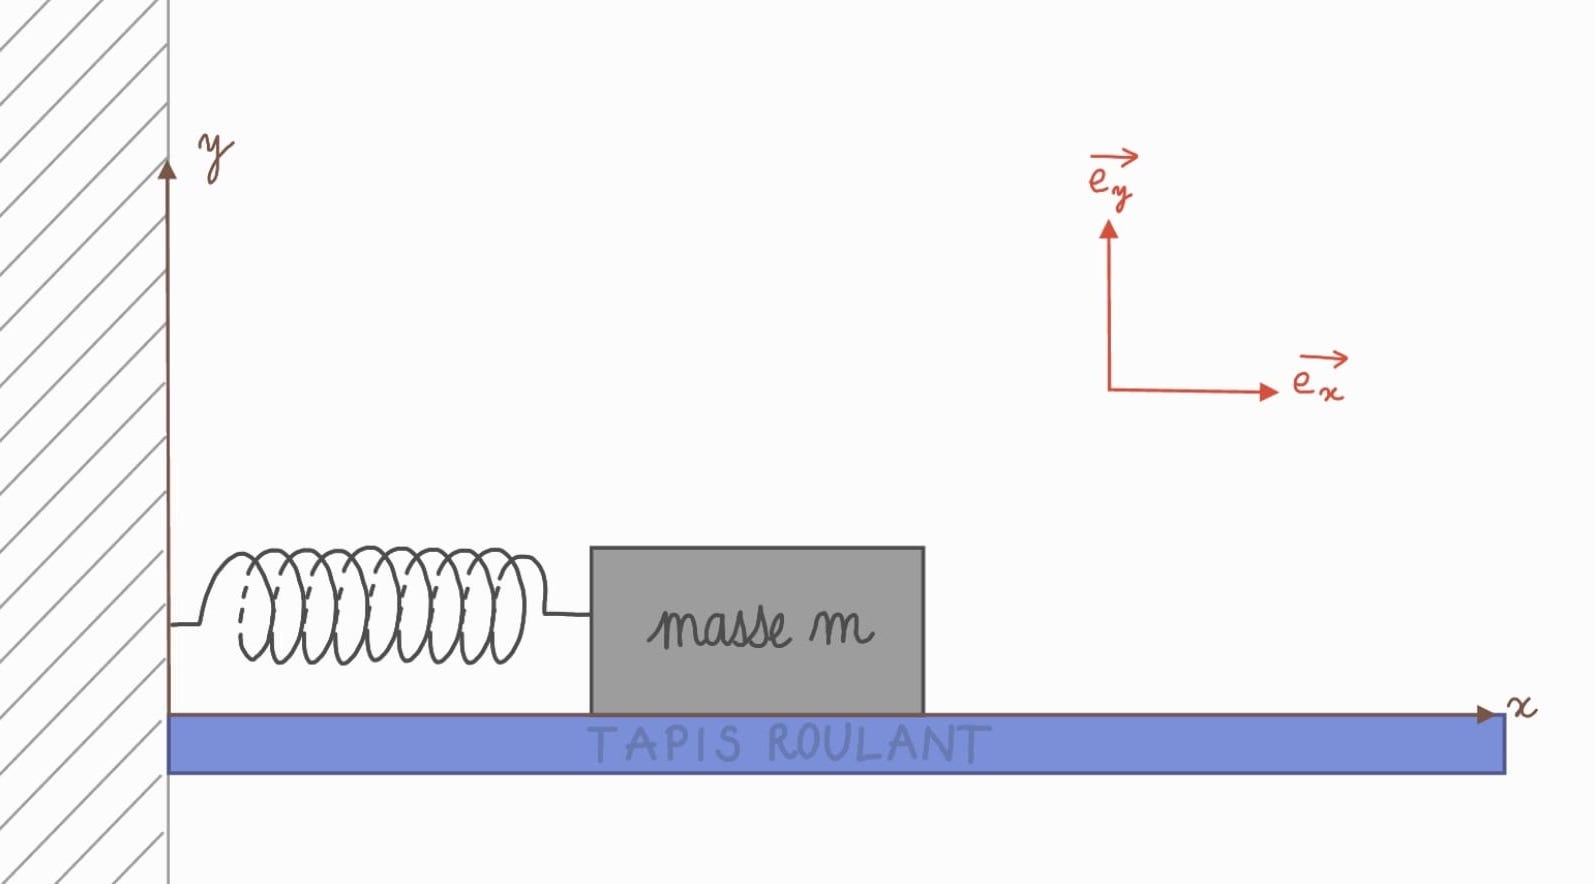
\includegraphics[scale=.26]{sch1.jpg}
	\caption{Système $\Sigma_1$}
\end{figure}
Dans ce chapitre nous allons modéliser la position de la masse en fonction du temps. Pour cela, nous allons présenter ultérieurement les 3 cas que l'on traitera.

\section{Introduction}\label{sec_1}
\paragraph{Variables du problème}\label{par_1.0.0.1}

\begin{adjustwidth}{0cm}{6cm}
\vspace{-.7cm}
\begin{alignat*}{2}
k \quad&[N\cdot m^{-1}] &&\quad \text{la raideur du ressort}\\
l_0  \quad&[m] &&\quad \text{la longueur du ressort} \\
m \quad&[g] && \quad\text{la masse du solide}\\
g \quad&[m\cdot s^{-2}] &&\quad \text{qui caractérise le champ gravitationnel} \\
\text{v} \quad& [m\cdot s^{-1}] && \quad\text{la vitesse du tapis roulant} \\
v_0 \quad& [m\cdot s^{-1}] && \quad\text{la vitesse initiale de la masse} \\
\nu \quad&[\text{sans unité}] && \quad\text{les frottements crées par le tapis roulant} 
\end{alignat*}
\end{adjustwidth}

%Dans notre étude, tous nos résultats seront selon ces six variables
\paragraph{Cinématique de la masse}\label{par_1.0.0.2}
\begin{alignat*}{3}
& \vv{OM} \quad && = \quad  x(t)~\vv{e_x}\\
\intertext{sa vitesse :}
& \vv{v}(M) \quad && = \quad  \dot{x}(t)~\vv{e_x}\\
\intertext{et son accélération :}
& \vv{a}(M) \quad && = \quad  \ddot{x}(t)~\vv{e_x}
\end{alignat*}

\paragraph{Efforts extérieurs}\label{par_1.0.0.3}
%
\begin{adjustwidth}{0cm}{3.5cm}
\vspace{-.7cm}
\begin{alignat*}{3}
& \vv{P} \quad && = \quad  -mg~\vv{e_y} &&\qquad \text{le Poids}\\
& \vv{R} \quad && = \quad  R~\vv{e_y} &&\qquad \text{la Réaction du tapis roulant}\\
& \vv{F_k} \quad && = \quad  -k(x(t)-l_0)~\vv{e_x} &&\qquad \text{la Force de rappel exercée par le ressort}\\
& \vv{F_{\ts{T}}} \quad && = \quad  F_{\ts{T}}~\vv{e_x} &&\qquad \text{la Force d'entraînement du tapis roulant}
\end{alignat*}
\end{adjustwidth}
%
\paragraph{Principe fondamental de la dynamique (Deuxième loi de Newton)}\label{par_1.0.0.4}
%
\begin{alignat}{2}
\sum{\vv{F}} &=  m\vv{a}\nonumber\\
\intertext{Suivant $\vv{e_y}$ :} \nonumber
 R- mg \quad & =  \quad 0 \nonumber\\
 R  \quad & = \quad  mg \nonumber\\
\intertext{Suivant $\vv{e_x}$ :} \nonumber \\
-k(x-l_0)+F_{\ts{T}}(t)\quad & = \quad m\ddot{x} \label{eq_1}
\end{alignat}
%
\subsection{Un système à deux régimes}\label{ssec_1.1}
Dans le mouvement de ce système, on distingue deux régimes spécifiques. Un premier régime, le régime d'adhérence ou la masse adhère à la surface du tapis roulant et est entrainée par celui-ci. Un second régime, le régime de glissement dans lequel la masse n'adhère plus au tapis roulant : elle glisse. Chacun de ces régimes est déterminé par des conditions particulières : on a à la fois des conditions initiales en position et en vitesse mais aussi une condition sur la force d'entraînement du tapis roulant sur l'ensemble de la phase sous ce régime. 

\subsubsection{Conditions sur les régimes}\label{sssec_1.1.1}

\paragraph{Régime d'adhérence}\label{par_1.1.1.1}
\mbox{}\\
Pour être en régime d'adhérence, les conditions initiales (à l'instant initial $t_d$ du régime) doivent respecter des contraintes particulières.
%
\begin{align*}
\begin{cases}
\vspace{.2cm}
x(t_d)\;=\; x_d\;=\; l,\quad l\in [l_0-\alpha~,~l_0+\alpha]\\
\dot{x}(t_d)\;=\;\text{v} 
\end{cases}
\end{align*}
%
Ici, l'intervalle $[l_0-\alpha~,~l_0+\alpha]$ est un intervalle particulier qui respecte les conditions d'adhérence. Plus précisément, si on se trouve à la position limite $l_0+\alpha$, le ressort est très tendu, donc au-delà de cette valeur, on passe à un régime de glissement ; à l'inverse, si on se trouve en $l_0-\alpha$, le ressort est très compressé donc ici encore, au-delà de cette valeur, on se trouve en régime de glissement. On verra dans la suite comment évaluer la valeur de $\alpha$.

De plus, la vitesse de la masse en régime d'adhérence correspond forcément à v, la vitesse d'entraînement du tapis roulant.   

On a aussi une condition sur la force d'entraînement du tapis sur l'ensemble du régime d'adhérence :
%
\begin{equation}
\mid F_{\ts{T}}(t) \mid  \quad<\quad F_c \quad=\quad\nu\; R \label{eq_2}
\end{equation}
%
\paragraph{Régime de glissement}\label{par_1.1.1.2}
\mbox{}\\
D'après ce qu'on a vu pour le régime d'adhérence, les conditions initiales pour se trouver en régime de glissement sont les conditions contraires aux conditions initiales d'adhérence :
%
\begin{align*}
\begin{cases}
\vspace{.2cm}
x(t_d)\;=\;x_d\;=\;l,\quad l\notin [l_0-\alpha~,~l_0+\alpha]\\
\dot{x}(t_d)\;=\;v_d\;\neq\; \text{v}
\end{cases}
\end{align*}
%
Ici, l'une des deux conditions suffit à être en régime de glissement (contrairement à précédemment où les deux conditions devaient être vérifiées).  

La condition sur l'ensemble de la phase pour la force est :
$$\mid F_{\ts{T}}(t)\mid\quad=\quad F_c$$
%
\subsubsection{Généralités sur le mouvement suivant le régime}\label{ssseq_1.1.2}
On va maintenant préciser l'équation du mouvement de la masse suivant le régime dans lequel elle se trouve. 

\paragraph{Régime d'adhérence}\label{par_1.1.2.1}
\mbox{}\\
Pour ce régime, la vitesse de la masse est constante et correspond à la vitesse du tapis roulant. On a donc :
\begin{alignat}{2}
& &\dot{x}(t)\quad & =\quad \text{v}~,\text{v}\in\mathbb{R} \nonumber\\
&\text{donc :} \quad & \ddot{x}(t)\quad & = \quad 0 \nonumber\\
&\text{et donc :} \quad & F_{\ts{T}}(t)\quad &= \quad k(x(t)-l_0) \quad \text{d'après le PFD} \nonumber\\
\intertext{En définissant $t_d$ comme l'instant initial du régime, on a finalement : }
& & \quad x(t) \quad &= \quad x(t_d)+(t-t_d)\;\text{v} \label{eq_3}
\end{alignat}
 %
\paragraph{Régime de glissement}\label{par_1.1.2.2}
\mbox{}\\
On cherche une expression de $x$ en fonction du temps en régime de glissement.D'après le PFD (vu précédemment), $x$ en régime de glissement est solution de l'équation différentielle qui suit :

\begin{equation}
m\ddot{x}(t)+kx(t)\quad=\quad k\;l_0 \pm F_c \label{eq_4}\\
\end{equation}

On résout cette équation différentielle. L'équation homogène associée est : 
\begin{alignat}{3}
& \quad & m\ddot{x}(t)+kx(t) \quad & = \quad 0 \label{eq_5}\\
& \Longleftrightarrow \quad & \ddot{x}(t)-\dfrac{k}{m}x(t)\quad & = \quad 0 \nonumber
\end{alignat}

Les solutions générales de cette équation \eqref{eq_5} sont :
%
\begin{align*}
x_h(t) \quad=\quad A\cos(\omega (t-t_d))+B\sin( \omega (t-t_d)) 
\end{align*}

Avec $A$, $B$ $\in \mathbb{R}$ et $\omega = \sqrt{\dfrac{k}{m}}$ et $t_d$ désignant l'instant initial du régime de glissement.  

On cherche maintenant une solution particulière de \eqref{eq_4}. Une solution évidente est : 

$$x_e(t)\quad =\quad l_0 \pm \dfrac{F_c}{k}$$

Donc l'ensemble des solutions de \eqref{eq_4} est :
\begin{align}
	x(t)& \quad=\quad x_h(t)+x_e(t)\nonumber\\
	&\quad=\quad A\cos(\omega (t-t_d))+B\sin (\omega (t-t_d)) +l_0 \pm \dfrac{F_c}{k} \label{eq_6}
\end{align}
Déterminons A et B.

Nous avons les conditions initiales suivantes : 

\begin{align*}
&\quad\begin{cases}
\vspace{.2cm}
	x(t_d)& \;=\; \quad x_d\\
	\dot{x}(t_d) & \;=\; \quad v_d 
\end{cases}
\\\\
\intertext{On rappelle que : 
$\dot{x}(t)=B\omega\cos(\omega (t-t_d) - A\omega \sin(\omega (t-t_d))$.
Donc en remplaçant $x(t_d)$ et $\dot x(t_d)$ par leur expressions, on obtient :}
\end{align*}
\begin{align*}
&\quad
\begin{cases}
\vspace{.2cm}
x(t_d) &= \quad A + l_0 \pm \dfrac{F_c}{k} = x_d \\
\dot{x}(t_d) &= \quad B\; \omega = v_d  
\end{cases}	\\\\
\Longleftrightarrow
&\quad
\begin{cases}
\vspace{.2cm}
A + l_0 \pm \dfrac{F_c}{k} \quad &= \quad x_d  \\
\hfill B\;\omega \quad &= \quad v_d 
\end{cases}	\\\\
\Longleftrightarrow
&\quad
\begin{cases}
\vspace{0.2cm}
	A \quad &= \quad x_d- \Big{(}l_0 \pm \dfrac{F_c}{k}\Big{)} \qquad(7)\\
	B  \quad &= \quad \dfrac{v_d}{\omega} \qquad \hfill(8)
\end{cases}	
\end{align*}

Si on injecte les expressions de $A$ et $B$ dans \eqref{eq_6}, on obtient :

\begin{align}
	x(t) \quad&=\quad A\cos(\omega (t-t_d))+B\sin(\omega (t-t_d))+ l_0 \pm \dfrac{F_c}{k} \nonumber \\
	&= \quad\left(x_d - \Big{(}l_0 \pm \dfrac{F_c}{k}\Big{)}\right)\cdot\cos(\omega (t-t_d)) +\dfrac{v_d}{\omega}\cdot\sin(\omega (t-t_d)) + l_0 \pm \dfrac{F_c}{k}\addtocounter{equation}{2} \label{eq_7}
\end{align}

\subsection{Cas traités}\label{ssec_1.2}
On va traiter quatre cas différents de phase initiale. Ces quatre cas constituent l'ensemble des possibilités pour les conditions initiales en $t_0$, instant initial du mouvement.  
\paragraph{Cas 1 (Régime initial d'adhérence)}\label{par_1.2.0.1}
\mbox{}\\
Le premier cas, le plus simple, est régi par les conditions initiales suivantes :
$$
\begin{cases}
	\vspace{.2cm}
	x_0\;\in\; [l_0-\alpha~,~l_0-\alpha]\\
	v_0 \;=\; \text{v}
\end{cases}
$$
C'est le seul cas pour lequel on débute par une phase d'adhérence. 

\paragraph{Cas 2 (Régime initial de glissement)}\label{par_1.2.0.2}
\mbox{}\\
Le deuxième cas représente le cas contraire au premier.$$
\begin{cases}
	\vspace{.2cm}
	x_0 \quad\text\small{quelconque}\qquad \text\small{ou}\\
	v_0 \quad\text\small{quelconque}
\end{cases}
$$
Il se divise en trois sous cas :
\subparagraph{Cas 2.1} \label{spar_1.2.0.2.1}
$$
\begin{cases}
	\vspace{.2cm}
	x_0  \in [l_0-\alpha~,~l_0-\alpha]\\
	v_0 \neq \text{v}
\end{cases}
$$
\subparagraph{Cas 2.2} \label{spar_1.2.0.2.2}
$$
\begin{cases}
	\vspace{.2cm}
	x_0  \not\in [l_0-\alpha~,~l_0-\alpha]\\
	v_0 = \text{v}
\end{cases}
$$

\subparagraph{Cas 2.3} \label{spar_1.2.0.2.3}
$$
\begin{cases}
	\vspace{.2cm}
	x_0  \not\in [l_0-\alpha~,~l_0-\alpha]\\
	v_0 \neq \text{v}
\end{cases}
$$
\newpage
\section{Démarche}\label{sec_2}
\subsection{Fonctions utilisées}\label{ssec_2.1}
Comme on a vu dans \ref{ssec_1.1} on a deux régimes, le régime d'adhérence et celui de glissement. On définit donc pour chacun des régimes une fonction de la position : 

\begin{lstlisting}
% Position dans un regime de glissement
function x = xG(t,t_d,x_d,v_d,v,omega,phi)
  x = (x_d - phi) * cos(omega * (t - t_d)) + v_d/omega * sin(omega * (t - t_d)) + phi;
endfunction
\end{lstlisting}

\begin{lstlisting}
% Position dans un regime d'adherence
function x = xA(t,t_d,x_d,v)
  x = v * (t - t_d) + x_d;
end
\end{lstlisting}

Dans les deux fonctions on a plusieurs arguments, \verb|t_d|, \verb|x_d|, \verb|v_d| qui sont des variables initiales au régime; v qui est la vitesse du tapis, enregistrée dans les variables d'entrée; finalement, on a \verb|omega| et \verb|phi| qui sont des variables intermédiaires. \\
\begin{lstlisting}
function [k,l_0,m,g,v,nu]=VarEntree
	k = 20;		% cst raideur ressort    	[N/m]
	l_0 = .3;	% long a vide ressort    	[m]
	m = .1;		% masse                  	[kg]
	g = 9.81;	% cst gravitation        	[m/s^2]
	v = .1;		% vitesse tapis          	[m/s]
	nu = 1;		% adherence tapis        	[]
endfunction
\end{lstlisting}

\begin{lstlisting}
function [F_c,omega,tcF,tcK]=VarInter(k,l_0,m,g,v,nu)
	F_c = nu*m*g;      % max Force entrainement					[N]
	omega = sqrt(k/m); % Pulsation									[1/s]
	tcF = F_c/(k*v);   % Temps carct deter par condition ini	[s]
	tcK = 2*pi/omega;  % Temps carct deter par pusation		[s]
endfunction
\end{lstlisting}

Le \verb|phi| utilisé dans la fonction \verb|xG| n'est pas une constante, on la définit comme $\varphi = l_0 \pm \dfrac{F_c}{k}$ avec le signe de $\dfrac{F_c}{k}$ dépendant de la différence de vitesse entre la masse et du tapis.

En effet, si la v$- v \geq 0$ alors v $\geq v$, c'est à dire que le tapis entraine la masse vers les x positifs. Ainsi on a $F_{\ts{T}}\geq0$. Dans le cas contraire, la masse a une vitesse plus élevée que celle du tapis et donc le tapis exerce une force vers les x négatifs. On aura donc $F_{\ts{T}}\leq0$.

Ainsi on définit une fonction \verb|Phi| qui dépend de la vitesse du tapis et celle de la masse au début de chacun des régimes.

\begin{lstlisting}
function phi = Phi(v_d,k,l_0,v,F_c)
  if(v_d != v)
    s = - sign(v_d - v);
  else
    s = 1;
  end
  phi = l_0 + s * F_c/k;
endfunction
\end{lstlisting}

\subsection{Recherche des temps de changement de régime}\label{ssec_2.2}
\subsubsection{Temps de passage : Adhérence $\rightarrow$ Glissement}\label{sssec_2.2.1}
On va dans un premier temps chercher l'instant $t$ tel qu'on passe de régime d'adhérence en régime de glissement. 

Comme on a vu dans \ref{par_1.1.1.1}, pour rester en régime d'adhérence, il faut satisfaire la condition \eqref{eq_2}. Ainsi, pour passer d'un régime d'adhérence à un régime de glissement il faut que: $\mid F_{\ts{T}}\mid = F_c$.

De fait, on définit la fonction \verb|fT| modélisant la force du tapis.
\begin{lstlisting}
function f = fT(t,t_d,x_d,v_d,v,k,l_0,F_c,re)
  if(v_d != v)
    s = - sign(v_d - v);
  else
    s = 1;
  end
  %
  if(re == 'ad')
    x = xA(t,t_d,x_d,v);
    f = k * (x - l_0);
  elseif(re == 'gl')
    f = s * F_c;
  end
end
\end{lstlisting}

On peut de la même manière définir la fonction \verb|fK| qui représente la force exercée par le ressort.
\begin{lstlisting}
function f = fK(t,t_d,x_d,v_d,v,k,l_0,omega,phi,re)
  if(re=='ad')
    x = xA(t,t_d,x_d,v);
  elseif(re=='gl')
    x=xG(t,t_d,x_d,v_d,v,omega,phi);
  end
   f = - k * (x - l_0);
endfunction
\end{lstlisting}

%Pour donner une estimation de $t$, on a deux options : par le calcul analytique (grâce à l'égalité \eqref{eq_3}) ou par un calcul de racine de la fonction $\mid F_{\ts T}\mid -\; F_c$.
%
%La relation \eqref{eq_3} nous permet de dire que 
%\begin{align}
%k(x_d+(t_{d+1}-t_d)\;\text{v}-l_0) \quad &= \quad F_c \nonumber\\
%\intertext{Et ainsi on a :}
%x_d+t_{d+1}\text{v}-t_d\text{v}-l_0 \quad &= \quad \dfrac{F_c}{k}\nonumber\\
%t_{d+1}\text{v}\quad &= \quad \dfrac{F_c}{k}-x_d+l_0+t_d\text{v}\nonumber\\
%t_{d+1}\quad &=\quad \dfrac{1}{v}\left(\dfrac{F_c}{k}-x_d+l_0+t_d\text{v}\right)\nonumber\\
%&=\quad t_d + \dfrac{F_c}{k\;\text{v}} - \dfrac{x_d - l_0}{\text{v}}
%\end{align}
Par définition, $\mid F_{\ts T}(t_1)\mid -\; F_c \; = \; 0$.  

Pour estimer $t_1$, on va donc effectuer numériquement une recherche de racine de $\mid F_{\ts T}\mid -\; F_c$. Pour effectuer cette recherche de racine, on va en réalité faire un calcul de minimum pour le carré de la fonction utilisée (le zéro sera ainsi bien le minimum). On va donc utiliser la fonction \verb|fminsearch()| qui permet d'obtenir ce minimum à partir d'un point de départ donné. Ce point de départ est assez important car il existe plusieurs racines et que l'on cherche la première racine positive (après $t_0$ sur l'axe des abscisses) ; il nous permet ainsi de tomber sur la racine attendue. On a donc le code suivant :
 
\begin{lstlisting}
%% SCRIPT PRINCIPAL
t01 = linspace(t_0,t_0 + 4*max(tcF,tcK),nt);

% Estimation numerique
CostA = @(t,t_d,x_d,v_d,v,k,l_0,F_c) (abs(fT(t,t_d,x_d,v_d,v,k,l_0,F_c,'ad')) - F_c).^2;
it1 = find(diff(sign(diff(CostA(t,t_0,x_0,v_0,v,k,l_0,F_c))))==2,1);
t_1 = fminsearch(@(t) CostA(t,t_0,x_0,v_0,v,k,l_0,F_c),t01(it1 + 1));
\end{lstlisting}
Avec \verb|x_0|, \verb|v_0|, \verb|t_0| les conditions initiales du régime d'adhérence, \verb|t_1| le temps de changement d'adhérence à glissement et \verb|t01| un vecteur de recherche arbitraire partant de $t_0$ suffisamment grand pour qu'il contienne $t_1$.

La fonction \verb|CostA| correspond au carré de $\mid F_{\ts T}\mid -\; F_c$.

\verb|it1| est le premier indice du vecteur \verb|t| pour lequel il y a un changement de signe de \verb|CostA| pour deux valeurs consécutives de \verb|t01| : on se place alors déjà très près du résultat recherché pour $t_1$ en prenant \verb|t01(it1+1)| comme point de départ de la recherche de $t_1$.   

\subsubsection{Temps de passage : Glissement $\rightarrow$ Adhérence}\label{sssec_2.2.2}
Pour passer d'un régime de glissement à un régime d'adhérence, on revient aux conditions pour être en régime d'adhérence (dans \ref{par_1.1.2.1}), en particulier, on a besoin que $\dot x = $ v.
Ainsi on définit une fonction \verb|vG| qui représente $\dot x$ en régime de glissement.
\begin{lstlisting}
function dot_x = vG(t,t_d,x_d,v_d,w,phi)
  dot_x = - (x_d - phi) * w * sin(w * (t - t_d)) + v_d * cos(w * (t - t_d));
endfunction
\end{lstlisting}

Par définition, le temps de passage de régime de glissement à régime d'adhérence vérifie :
\begin{alignat*}{2}
 &\dot{x}(t_1)\; &=\;\text{v}\\
\Longleftrightarrow \quad & \dot{x}(t_1)-\text{v}\;&=\;0
\end{alignat*}

De manière analogue à ce que l'on a fait précédemment pour $t_1$ on va trouver numériquement une approximation de la racine de la fonction $\dot x(t) -$v.

\begin{lstlisting}
%% SCRIPT PRINCIPAL
t01 = linspace(t_1,t_1 + 4*max(tcK,tcF),nt);

% Estimation numerique
CostG = @(t,t_d,x_d,v_d,w,phi,v) ((vG(t,t_d,x_d,v_d,w,phi) - v).^2);
it1 = find(diff(sign(diff(CostG(t01,t_0,x_0,v_0,w,phi,v))))==2,1);

t_1 = fminsearch(@(t) CostG(t,t_0,x_0,v_0,w,phi,v),t01(it+1));
\end{lstlisting}

Avec, à nouveau, \verb|x_0|, \verb|v_0|, \verb|t_0| les conditions initiales du régime de glissement, \verb|t_1| le temps de changement de glissement à adhérence et \verb|t01| un vecteur de recherche partant de $t_0$ et de longueur arbitraire suffisamment grande pour contenir $t_1$.

La fonction \verb|CostG| correspond au carré de $\dot x(t) -$v dont on effectue une recherche de minimum avec la fonction \verb|fminsearch| (ce qui une nouvelle fois correspond à trouver une racine de $\dot x(t) -$v). 

\verb|t01(it1+1)| est le point de départ de cette recherche de minimum. Celui-ci est déterminé par le calcul de l'indice particulier \verb|it1| qui est l'indice d'une différence entre deux valeurs consécutives de \verb|CostG| calculé pour le  vecteur \verb|t01| de recherche. Ici encore, l'indice \verb|it1+1| nous permet d'être très proche de $t_1$ et ainsi optimiser la recherche du \verb|fminsearch|.

\newpage
\section{Cas 1}
On cherche à caractériser le mouvement de la masse, sa vitesse et la force d'entraînement du tapis en fonction du temps et d'en donner une représentation graphique dans le premier cas. Pour cela, on va d'abord déterminer les premiers temps $t_n$ de changement de régime.   
  
Comme énoncé précédemment, on se trouve dans les conditions initiales suivantes : 

$$
\begin{cases}
	\vspace{.2cm}
	x_0\in [l_0-\alpha~,~l_0-\alpha]\\
	v_0 = \text{v}
\end{cases}
$$

Le premier régime est alors un régime d'adhérence. Dans le code, on initialise de la même façon les variables initiales : 
\begin{lstlisting}
%% Variables d'initialisation
t_0 = 0 			% tmps ini		[s]
x_0 = l_0; 		% position ini	[m]
v_0 = v;			% vitesse ini	[m/s]       
\end{lstlisting}

Dans la suite du code, on utilisera toujours v directement. 


\subsection{Calcul de $t_1$ : Adhérence $\rightarrow$ Glissement}\label{ssec_3.1}
On va dans un premier temps chercher l'instant $t_1$ auquel le système va passer en régime de glissement. Comme on l'a montré précédemment en \ref{ssec_2.2} on va calculer une estimation de $t_1$ en cherchant numériquement une racine de $\mid F_{\ts T}\mid -\; F_c$ :

\begin{lstlisting}
%% SCRIPT main1
t01 = linspace(t_0,t_0 + 4*max(tcK,tcF),nt);

CostA = @(t,t_d,x_d,v_d,v,k,l_0,F_c) (abs(fT(t,t_d,x_d,v_d,v,k,l_0,F_c,'ad') - F_c).^2);
it1 =find(diff(sign(diff(CostA(t01,t_0,x_0,v_0,v,k,l_0,F_c))))==2,1);

t_1 = fminsearch(@(t) CostA(t,t_0,x_0,v_0,v,k,l_0,F_c),t01(it1+1))
\end{lstlisting}

On effectue dans le même temps le calcul de $x_1$ avec la valeur de $t_1$ que l'on a calculée. On obtient le résultat suivant :

\begin{lstlisting}
x_1 = xA(t_1,t_0,x_0,v_0) 
%ou = xG(t_1,t_0,x_0,v_0,w,phi) par continuite de x
\end{lstlisting}


\begin{lstlisting}
octave > main1
t_1 = 0.4905
x_1 = 0.3491
\end{lstlisting}


\subsection{Calcul de $t_2$ : Glissement $\rightarrow$ Adhérence}
On passe ensuite en régime de glissement. On cherche maintenant à calculer $t_2$ . Ici encore, on utilise la méthode vue en \ref{ssec_2.2} pour déterminer $t_2$ : on effectue un calcul de racine pour $\dot{x}-\text{v}$. On a alors le code suivant :

\begin{lstlisting}
%% SCRIPT main1
t12 = linspace(t_1,t_1 + 2*max(tcF,tcK),nt);

CostG = @(t,t_d,x_d,v_d,w,phi,v) ((vG(t,t_d,x_d,v_d,w,phi) - v).^2);
it2 = find(diff(sign(diff(CostG(t12,t_1,x_1,v_1,w,phi,v))))==2,1);

t_2 = fminsearch(@(t) CostG(t,t_1,x_1,v_1,w,phi,v),t12(it2+1))
\end{lstlisting}

Le choix de point de départ de recherche \verb|t_1 + tcK| dans le \verb|fminsearch(...)| est à nouveau choisi de sorte qu'il soit assez proche de $t_2$. 

On effectue également le calcul de $x$ associé à $t_2$ :

\begin{lstlisting}
x_2 = xG(t_2,t_1,x_1,v,v,omega,phi)
\end{lstlisting}

A ce stade on a :

\begin{lstlisting}
octave > main1
t_1 = 0.4905
x_1 = 0.3491
t_2 = 0.9348
x_2 = 0.3491
\end{lstlisting}

On remarque que $x_1=x_2$.

\subsection{Calcul de $t_3$}
On répète l'opération pour $t_3$ : on passe en régime d'adhérence après $t_2$ et on effectue le calcul de $t_3$  de la même manière que l'on a fait le calcul de $t_1$. 
\begin{lstlisting}
%% SCRIPT main1
t23 = linspace(t_2,t_2 + 4*max(tcK,tcF),nt);

it3 = find(diff(sign(diff(CostA(t23,t_2,x_2,v_2,v,k,l_0,F_c))))==2,1);

t_3 = fminsearch(@(t) CostA(t,t_2,x_2,v_2,v,k,l_0,F_c),t23(it3+1))
\end{lstlisting}
 
\subsection{Représentation graphique et résultats}
On a les valeurs suivantes pour $t_0$, $t_1$, $t_2$, $t_3$ :
\begin{lstlisting}
octave> main1
 t_0 = 0
 t_1 = 0.3270
 t_2 = 0.6898
 t_3 = 0.6898
\end{lstlisting}

\begin{figure}[h!]
  \centering
  \hspace{-2cm}
  \begin{subfigure}[b]{.45\linewidth}
    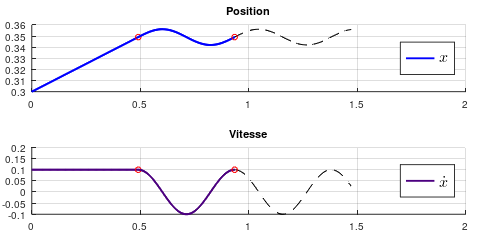
\includegraphics[width=1.3\linewidth]{Cas1a.png}
  \end{subfigure}
  \hspace{2cm}
  \begin{subfigure}[b]{.45\linewidth}
    \includegraphics[width=1.3\linewidth]{CAS1b.png}
  \end{subfigure}
  \caption{Cas 1 ; $x_0 = l_0$ , $v_0 = \text{v}$}
\end{figure}

On remarque ici que $t_2 = t_3$. On peut donc dire qu'après $t_2$ on passe en régime de glissement sans revenir au régime d'adhérence. En effet, la condition $F_{\ts{T}} = F_c$ est toujours vérifiée, donc aussitôt qu'on rentre en régime d'adhérence, on en sort.

On a donc les représentations graphiques suivantes pour le mouvement, la vitesse et les forces d'entraînement du tapis et de réaction du ressort : 

\newpage
\section{Cas 2}
Jusqu'à ici nous avons vu que les fonctions \verb|CostG| et \verb|CostA| ont un minimum local aux temps de changement de régimes. Avec le Cas 1 on retrouve toujours un même patron, peu importe les conditions initiales appartenant au cas 1, en effet on commence en régime d'adhérence puis on passe en régime de glissement indéfiniment.

La question qu'on pourrait se poser est "Est ce qu'on voit ce phénomène aussi quand on change de cas"?


Comme vu dans \ref{ssec_1.2} le cas 2 regroupe tous les cas possibles qui sont contraires au premier. Même si les cas 2.1, 2.2 et 2.3 n'ont pas les mêmes conditions initiales, ils suivent le même modèle.\\
Ainsi, pour étudier chacun des cas nous faisons une fonction qui renvoie les temps et position de changement de passage en fonction des conditions initiales.

\begin{lstlisting}
function lst = List(min_x,max_x,min_v,max_v,nx,nv,k,l_0,m,g,v,nu,F_c,w,tcF,tcK)
  lst = [];
  nt = 200;
  t_0 = 0;
  
  x0 = linspace(min_x,max_x,nx);
  v0 = linspace(min_v,max_v,nv);

  for i = 1:nx;
    x_0 = x0(i);
    
    for j = 1:nv;
      v_0 = v0(j);
      %%Phase 1 : glissement ----------------------
      phi = Phi(v_0,k,l_0,v,F_c);
      t01=linspace(t_0,t_0 + 4*max(tcF,tcK),nt);
      CostG = @(t,t_d,x_d,v_d,w,phi,v) ((vG(t,t_d,x_d,v_d,w,phi) - v).^2);
      it1=find(diff(sign(diff(CostG(t01,t_0,x_0,v_0,w,phi,v))))==2,1);
      
      t_1 = fminsearch(@(t) CostG(t,t_0,x_0,v_0,w,phi,v),t01(it1+1));
      x_1 = xG(t_1,t_0,x_0,v_0,w,phi);
      
      %% Phase 2 : adherence ------------------------
      v_1 = v;
      phi = Phi(v_1,k,l_0,v,F_c);
      t12 = linspace(t_1,t_1 + 4*max(tcK,tcF),nt);      
      CostA = @(t,t_d,x_d,v_d,v,k,l_0,F_c) (abs(fT(t,t_d,x_d,v_d,v,k,l_0,F_c,'ad') - F_c).^2);
      it2 = find(diff(sign(diff(CostA(t12,t_1,x_1,v_1,v,k,l_0,F_c))))==2,1);

      if(length(it2)<1)
            continue
      end

      t_2 = fminsearch(@(t) CostA(t,t_1,x_1,v_1,v,k,l_0,F_c),t12(it2+1));
      x_2 = xA(t_2,t_1,x_1,v_1);
      
      %% Phase 3 : glissement ------------------------
      v_2 = v;
      phi = Phi(v_2,k,l_0,v,F_c);
      t23 = linspace(t_2,t_2 + 2*max(tcF,tcK),nt);
      it3 = find(diff(sign(diff(CostG(t23,t_2,x_2,v_2,w,phi,v))))==2,1);
      
      t_3 = fminsearch(@(t) CostG(t,t_2,x_2,v_2,w,phi,v),t23(it3+1));
      x_3 = xG(t_3,t_2,x_2,v_2,w,phi);

      lst = [lst;x_0,v_0,t_1,t_2,t_3,t_2-t_1];%X_1,x_2,x_3];
    end
  end
endfunction
\end{lstlisting}

\subsection{Observations}
\subsubsection{Cas 2.1}
Voici les conditions initiales qu'on doit suivre:
$$
\begin{cases}
	\vspace{.2cm}
	x_0 \in [l_0-\alpha~,~l_0-\alpha]\\
	v_0\neq \text{v}
\end{cases}
$$
On peut donc écrire :
\begin{lstlisting}
List(l_0,l_0,-1,1,1,21,k,l_0,m,g,v,nu,F_c,w,tcF,tcK)
\end{lstlisting}

Ce qui nous donne le tableau suivant :

\begin{figure}[h!]
	\centering
	\renewcommand{\arraystretch}{1.5}
	\begin{tabular}{|C{1.3cm}|C{1.3cm}|C{1.3cm}|C{1.3cm}|C{1.3cm}|C{1.3cm}|C{1.3cm}|C{1.3cm}|C{1.3cm}|}
	\hline
	$x_0$ & $v_0$ & $t_1$ & $t_2$ & $t_3$ & $t_2-t_1$ & $x_1$ & $x_2$ & $x_3$ \\
	\hline
	0.3000 & -1.0000 & 0.0740 & 0.9317 & 1.3759 & 0.8577 & 0.2633 & 0.3491 & 0.3490\\
	\hline
	0.3000 & -0.9000 & 0.0708 & 0.8712 & 1.3155 & 0.8004 & 0.2690 & 0.3490 & 0.3491\\
	\hline
	0.3000 & -0.8000 & 0.0672 & 0.8126 & 1.2569 & 0.7454 & 0.2745 & 0.3491 & 0.3491\\
	\hline
	0.3000 & -0.7000 & 0.0631 & 0.7563 & 1.2006 & 0.6932 & 0.2797 & 0.3490 & 0.3491\\
	\hline
        0.3000 & -0.6000 & 0.0582 & 0.7028 & 1.1471 & 0.6446 & 0.2846 & 0.3491 & 0.3491\\
        \hline
        0.3000 & -0.5000 & 0.0525 & 0.6530 & 1.0972 & 0.6005 & 0.2890 & 0.3491 & 0.3491\\
        \hline
        0.3000 & -0.4000 & 0.0458 & 0.6076 & 1.0519 & 0.5618 & 0.2929 & 0.3490 & 0.3491\\
        \hline
        0.3000 & -0.3000 & 0.0383 & 0.5679 & 1.0122 & 0.5297 & 0.2961 & 0.3490 & 0.3490\\
        \hline
        0.3000 & -0.2000 & 0.0297 & 0.5352 & 0.9795 & 0.5055 & 0.2985 & 0.3490 & 0.3491\\
        \hline
        0.3000 & -0.1000 & 0.0203 & 0.5107 & 0.9550 & 0.4905 & 0.3000 & 0.3490 & 0.3490\\
        \hline
        0.3000 &       0 & 0.0102 & 0.4956 & 0.9399 & 0.4854 & 0.3005 & 0.3490 & 0.3490\\
        \hline
        0.3000 &  0.2000 & 0.0100 & 0.4855 & 0.9298 & 0.4754 & 0.3015 & 0.3491 & 0.3491\\
        \hline
        0.3000 &  0.3000 & 0.0195 & 0.4707 & 0.9151 & 0.4513 & 0.3039 & 0.3490 & 0.3491\\
        \hline
        0.3000 &  0.4000 & 0.0281 & 0.4474 & 0.8916 & 0.4193 & 0.3071 & 0.3491 & 0.3490\\
        \hline
        0.3000 &  0.5000 & 0.0359 & 0.4164 & 0.8607 & 0.3805 & 0.3110 & 0.3490 & 0.3490\\
        \hline
        0.3000 &  0.6000 & 0.0427 & 0.3790 & 0.8233 & 0.3364 & 0.3154 & 0.3491 & 0.3491\\
        \hline
        0.3000 &  0.7000 & 0.0487 & 0.3364 & 0.7807 & 0.2878 & 0.3203 & 0.3491 & 0.3491\\
        \hline
        0.3000 &  0.8000 & 0.0539 & 0.2895 & 0.7338 & 0.2356 & 0.3255 & 0.3491 & 0.3491\\
        \hline
        0.3000 &  0.9000 & 0.0584 & 0.2391 & 0.6833 & 0.1806 & 0.3310 & 0.3491 & 0.3491\\
        \hline
        0.3000 &  1.0000 & 0.0624 & 0.1857 & 0.6300 & 0.1233 & 0.3367 & 0.3490 & 0.3491\\
        \hline
	\end{tabular}
        \caption{Cas 2.1 ; $x_0 = l_0$ , $v_0 \in [- 1,+ 1]_{v \neq \text{v}}$}

\end{figure}

En premier, une chose nous saute aux yeux : $x_2$ et $x_3$ ont les mêmes valeurs à un milimètre près pour un $v_0$ quelconque.
On peut remarquer également que $t_2$ et $t_3$ a un écart constant pour chacun des $v_0$. On peut se demander qu'arrive donc entre $t_1$ et $t_2$.

%%% GRAPHIQUE %%%
On peut remarquer que plus la vitesse est élevée, plus $t_1$ et $t_2$ sont proches. Ainsi, lors qu'on soumet la masse à  une vitesse initiale très élevée on a un régime d'adhérence presque inpersceptible (image de gauche). Au contraire si on prend une vitesse initiale négative on retrouvera un régime d'adhérence beaucoup plus imposant (graphique de droite).
\begin{figure}[h!]
  \centering
  \hspace{-3cm}
  \begin{subfigure}[b]{.4\textwidth}
    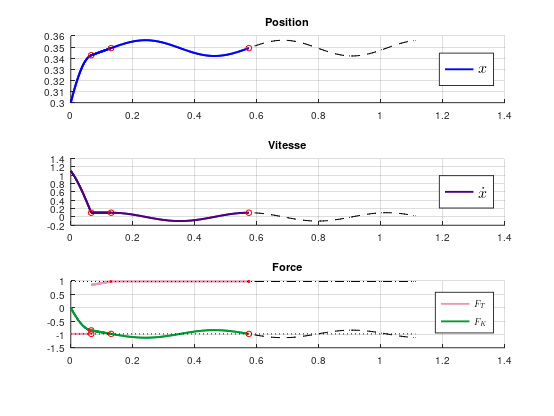
\includegraphics[width = 1.5\linewidth]{CAS2_1a.png}
  \end{subfigure}
  \hspace{2.5cm}
  \begin{subfigure}[b]{.4\textwidth}
    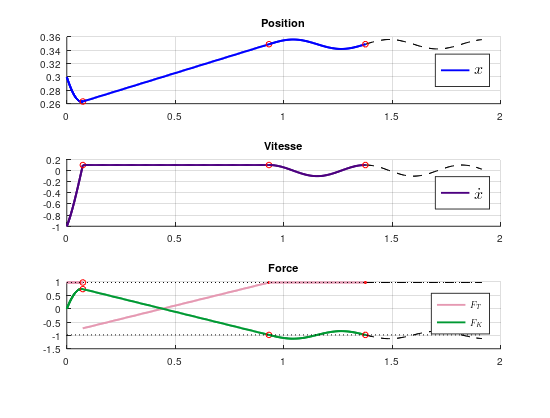
\includegraphics[width = 1.5\linewidth]{CAS2_1b.png}
  \end{subfigure}
  \caption{Cas 2.1 pour $v_0 = 1.1$ et $v_0 = -1.0$}
\end{figure}

Pour visualiser plus cette relation, on représente $t_1$ et $t_2 - t_1$ en fonction de $v_0$ :

\begin{figure}[h!]
  \centering
  \begin{subfigure}[b]{.4\textwidth}
    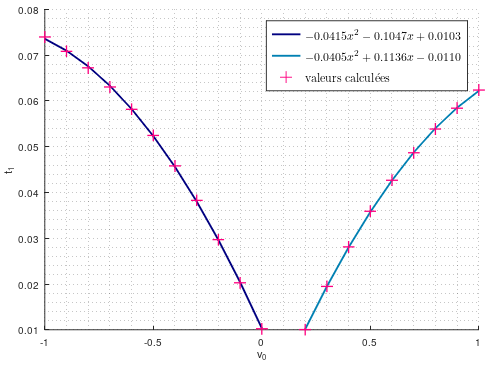
\includegraphics[width = \linewidth]{t_1.png}
    \caption*{$t_1-t_0$ en fonction de $v_0$}
  \end{subfigure}
  \hspace{1cm}
  \begin{subfigure}[b]{.4\textwidth}
    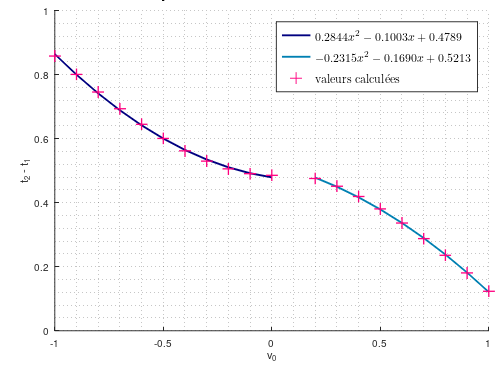
\includegraphics[width = \linewidth]{t_2-t_1.png}
    \caption*{$t_2-t_1$ en fonction de $v_0$}
  \end{subfigure}
  \caption{Differences de temps de changement de régimes en fonction de $v_0$}
\end{figure}

On peut voir que plus les conditions initiales sont proches des conditions d'adhérence, plus on trouve un $t_1$ proche de 0, et donc on se rapproche du cas 1.

\subsubsection{Cas 2.2}
On change de conditions initiales, maintenant on a:

$$
\begin{cases}
	\vspace{.2cm}
	x_0 \not\in [l_0-\alpha~,~l_0-\alpha]\\
	v_0 = \text{v}
\end{cases}
$$

\begin{lstlisting}
  List(l_0,l_0 + .3,v,v,30,1,k,l_0,m,g,v,nu,F_c,w,tcF,tcK)
\end{lstlisting}

\begin{figure}[h!]
	\centering
	\renewcommand{\arraystretch}{1.5}
	\begin{tabular}{|C{1.3cm}|C{1.3cm}|C{1.3cm}|C{1.3cm}|C{1.3cm}|C{1.3cm}|C{1.3cm}|C{1.3cm}|C{1.3cm}|}
	  \hline
       	  $x_0$ & $v_0$ & $t_1$ & $t_2$ & $t_3$ & $t_2-t_1$ & $x_1$ & $x_2$ & $x_3$ \\
          \hline                                                                                       
          0.351724 & 0.100000 & 0.393151 & 0.419921 & 0.864200 & 0.026770 & 0.346375 & 0.349052 & 0.349051\\
          \hline
          0.362069 & 0.100000 & 0.292483 & 0.422729 & 0.867008 & 0.130246 & 0.336028 & 0.349053 & 0.349052\\
          \hline
          0.372414 & 0.100000 & 0.263699 & 0.497331 & 0.941610 & 0.233632 & 0.325685 & 0.349049 & 0.349048\\
          \hline
          0.382759 & 0.100000 & 0.251398 & 0.588445 & 1.032743 & 0.337047 & 0.315343 & 0.349047 & 0.349048\\
          \hline
          0.393103 & 0.100000 & 0.244651 & 0.685207 & 1.129495 & 0.440556 & 0.304997 & 0.349052 & 0.349052\\
          \hline
          0.403448 & 0.100000 & 0.240407 & 0.784378 & 1.228721 & 0.543970 & 0.294650 & 0.349047 & 0.349052\\
          \hline
          0.413793 & 0.100000 & 0.237539 & 0.884956 & 1.329273 & 0.647418 & 0.284308 & 0.349050 & 0.349053\\
          \hline
          0.424138 & 0.100000 & 0.235402 & 0.986296 & 1.430575 & 0.750893 & 0.273960 & 0.349049 & 0.349048\\
          \hline
          0.434483 & 0.100000 & 0.233815 & 1.088176 & 1.532406 & 0.854361 & 0.263617 & 0.349053 & 0.349047\\
          \hline
          0.444828 & 0.100000 & 0.232595 & 1.190325 & 1.634592 & 0.957731 & 0.253275 & 0.349048 & 0.349046\\
          \hline
          0.455172 & 0.100000 & 0.231525 & 0.311803 & 0.523778 & 0.080278 & 0.242925 & 0.250953 & 0.447148\\
          \hline
          0.465517 & 0.100000 & 0.230731 & 0.414396 & 0.626371 & 0.183665 & 0.232584 & 0.250950 & 0.447150\\
          \hline
          0.475862 & 0.100000 & 0.229999 & 0.517139 & 0.729114 & 0.287140 & 0.222236 & 0.250950 & 0.447151\\
          \hline
          0.486207 & 0.100000 & 0.229449 & 0.619976 & 0.831951 & 0.390527 & 0.211895 & 0.250948 & 0.447153\\
          \hline
          0.496552 & 0.100000 & 0.228900 & 0.722964 & 0.934938 & 0.494063 & 0.201546 & 0.250953 & 0.447148\\
          \hline
          0.506897 & 0.100000 & 0.228473 & 0.825923 & 1.037897 & 0.597450 & 0.191203 & 0.250948 & 0.447152\\
          \hline
          0.517241 & 0.100000 & 0.228107 & 0.928971 & 1.140946 & 0.700865 & 0.180861 & 0.250947 & 0.447154\\
          \hline
          0.527586 & 0.100000 & 0.227740 & 1.032092 & 1.244067 & 0.804351 & 0.170514 & 0.250949 & 0.447152\\
          \hline
          0.537931 & 0.100000 & 0.227435 & 1.135252 & 1.347227 & 0.907817 & 0.160169 & 0.250951 & 0.447150\\
          \hline
          0.548276 & 0.100000 & 0.227191 & 1.238451 & 1.450426 & 1.011260 & 0.149827 & 0.250953 & 0.447148\\
          \hline
          0.558621 & 0.100000 & 0.226886 & 1.341641 & 1.553616 & 1.114755 & 0.139477 & 0.250952 & 0.447149\\
          \hline
          0.568966 & 0.100000 & 0.226703 & 1.444833 & 1.656808 & 1.218130 & 0.129136 & 0.250949 & 0.447152\\
          \hline
          0.579310 & 0.100000 & 0.226459 & 1.548077 & 1.760052 & 1.321618 & 0.118787 & 0.250949 & 0.447152\\
          \hline
          0.589655 & 0.100000 & 0.226276 & 1.651326 & 1.863300 & 1.425050 & 0.108442 & 0.250947 & 0.447153\\
          \hline
          0.600000 & 0.100000 & 0.226153 & 1.754666 & 1.966641 & 1.528512 & 0.098103 & 0.250954 & 0.447147\\
          \hline
	\end{tabular}
        \caption{Cas 2.2 ; $x_0 \in [0.3,0.6]$ , $v_0 = v$}

\end{figure}
\end{document}
